\subsection{Les 13 nains de berkeley}
La collection des {\em 13 nains de Berkeley}\cite{dwarfs} est une méthode de classification des problèmes en fonction de leurs motifs de calculs et de communications.
%
Il est intéressant de voir si Taggre peut répondre aux 13 problèmes et si c'est le cas quelle serait la stratégie d'agrégation à utiliser.
%
En effet, le choix des opérateurs dans Taggre se fait à l'appréciation du programmeur.
%
Malheureusement, tous les problèmes ne se prêtent pas à cet exercice.
%
Certaines classes de problèmes ne peuvent pas se paralléliser avec du parallélisme à base de graphes de tâches, ou ne présentent aucun intérêt à être paralléliser de cette façon (MapReduce, Graph Traversal, Dynamic Programming, Backtrack and Branch-and-Bound, Graphical Models et Finite State Machines).
%
Les problèmes rencontrés en algèbre linéaire dense sont souvent réguliers et le programmeur peut facilement choisir une granularité.
%
La classe de problème {\em structured grids} peut être parallélisée avec du parallélisme à base de graphe de tâches, mais il ne s'agit pas du meilleur paradigme de parallélisation pour cette classe.
%
La même réflexion peut être faite pour la classe de problème {\em unstructured grids}.


La classe de problème {\em combinational logic} s'apparente à du parallélisme d'instructions.
%
Cette granularité est trop faible pour être traitée par un ordonnanceur de tâches logiciel.

Il ne reste donc plus que trois classes de problème pouvant utiliser Taggre, l'algèbre linéaire creuse, les méthodes N-Body et les méthodes spectrales.
%
L'algèbre linéaire creuse comporte un ensemble très vaste d'algorithmes qui ne se parallélisent pas tous de la même manière.
%
Dans ce manuscrit, nous étudierons la parallélisation du produit matrice vecteur creux et de la factorisation ILU.


\subsubsection{Méthodes N-Body}
Les méthodes N-Body consistent à simuler les interactions entre particules dans un espace au cours du temps.
%
Chaque particule aura un état particulier (masse, position, vitesse ...) et chaque interaction aura pour effet de changer cette état.
%
Pour chaque pas de temps, il faut mettre à jour chaque particule en fonction de l'état des autres particules.
%
Le calcul exact étant trop coûteux (complexité en O($n^2$)), il existe des heuristiques.
%
L'une d'entre elles consiste à diviser l'espace en plusieurs sous-espaces et de seulement simuler exactement les interactions des particules du même sous-espace et faire une approximation des particules pour les interactions avec celles d'un autre sous espace.
%
Des travaux de recherche se sont concentrés à traiter ce problème avec des graphes de tâches\cite{scalfmm}, et comme le graphe est un arbre, ils ont eux-même fait de l'agrégation de noeuds pour obtenir une bonne granularité.
%
Taggre n'est donc pas utile dans ce cas, le problème de granularité étant déjà traiter par le programmeur.


\subsubsection{Méthodes spectrales}
Dans le cas des méthodes spectrales, le graphe représentant le parallélisme est plus large que haut.
%
Le motif du graphe est en papillon, nous avons donc beaucoup de connexions entre chaque niveau du graphe, l'opérateur F pourra s'occuper de regrouper les tâches d'un même niveau ensemble.
%
Celui-ci nous permettra de diminuer le nombre de tâches en diminuant le parallélisme (Fig.\ref{fig:dwarf_spec}).
%
Pour évaluer le gain lié à l'agrégation, nous allons utiliser le simulateur de Taggre avec les paramètres 0,9 pour les effets de cache et 5 pour le coût d'ordonnancement.
%
La hauteur du graphe sera le logarithme en base 2 du nombre de tâches par niveau.
%
La table~\ref{tab:spectral} nous montre les gains obtenus en utilisant différents opérateurs d'agrégation.
%
Les opérateurs D et F offrent presque les mêmes performances.
%
Si les paramètres du simulateur sont corrects (très petites tâches) alors l'agrégation permettra de diviser le temps de calcul par 6.


%   (-_-)   %
\begin{figure}
  \centering
  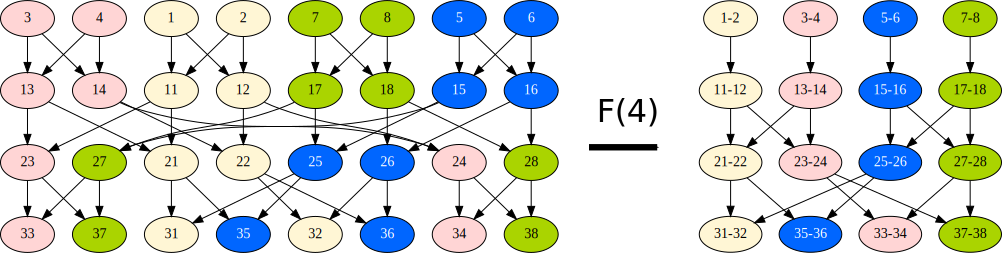
\includegraphics[width=\textwidth]{dwarf_spec}
  \caption{Exemple d'agrégation sur un graphe de méthode spectrale.}
  \label{fig:dwarf_spec}
\end{figure}
%   (-_-)   %
\begin{center}
  \begin{tabular}{|l|c|c|c|c|c|c|c|c|}
    \hline
   Nombre de tâches &  \multicolumn{8}{c|}{Types d'agrégations}\\
   par niveau & \O & F(6) & F(12) & F(24) & D(8) & D(16) & D(32) & D(64) \\
    \hline
   32768 & 262146 & 108246 & 51714 & 39487 & 70425 & 55788 & 40980 & 46409 \\
   1024  & 1690   & 2162   & 937   & 903   & 1035  & 965   & 899   & 1033 \\
    \hline
  \end{tabular}
  \captionof{table}{Résultats du simulateur d'exécution de tâches sur un graphe typique des méthodes spectrales.}
  \label{tab:spectral}
\end{center}
%% RES 15 niveau
%% 0    262146
%% F 12 51714.9
%% F 24 39487.8
%% F 6  108246
%% D 8  70425
%% D 16 55788.5
%% D 32 40980
%% D 64 46409.6
%% RES 10 niveau
%% 0    1690
%% F 12 937
%% F 24 903
%% F 6  2162
%% D 8  1035
%% D 16 965
%% D 32 899
%% D 64 1033
%\subsubsection{Les arbres}

